%!TEX root = ../main.tex
% !TeX encoding = UTF-8
\section{Design de Sistemas Wearables} \label{chap:design}

   A seguir, serão descritos alguns tópicos seguindo conceitos estabelecidos por vários trabalhos como \cite{Arato2003, Arato2005, Mann2007, Hassine2017, Sass2010}.
   %Esses tópicos são necessários para o entendimento básico dos arcabouços metodológicos de \codesign\ e o seu particionamento para sistemas embarcados, em especial para sistemas \wearables, além de definições matemáticas sobre.

   %Os tópicos a seguir são a Definição de \Design\ de Referência de \Software\ (Seção~\ref{sec:GCF}) bem como o Ganho de Performance (Seção~\ref{sec:ganho_performance}) em tais sistemas, o Particionamento \HS\ para Sistemas \Wearables\  (Seção~\ref{sec:desenvolvimento}) e a Proposta de Procedimento Analítico (Seção~\ref{sec:proposta}).

   \subsection{Design Referencial de Software} \label{sec:GCF}

      Segundo \cite{Sass2010}, é possível descrever sistemas, livre de especificações formais de \software\ ou \hardware\ por meio de descrições de protótipos simples, conhecidos como \design\ referencial de \software\ (DRS).
      %Com ele, é possível ter uma generalização de uma especificação sistêmica, eliminando quaisquer tipo de incertezas sobre o comportamento do sistema ao realizar uma análise sobre, sendo este podendo ser representado por diversas formas.
      % além de outras como o fato de que sua especificação pode ser analisada por ferramentas computacionais, e gerando modelos aut.

      %Assumindo que o \design\ de referência de \textit{software} já exista,
      %Primeiramente, será demonstrado matematicamente como computação está em \design\ referencial de \sof%htware\ para que depois, isso possa nos auxiliar na decisão do que deverá ser implementado em nível de \hs.
      Como o algoritmo a ser analisado e particionado também pode ser representado em forma de grafo de tarefas/rotinas, pode-se então associar o \design\ da sub-rotina também com o uso da teoria de grafos \cite{Mann2007}, em especial o Grafo de Controle de Fluxo (GCF).
      Ele é definido por $C = (B, F) \label{eq:subrotina}$
      %\begin{equation}
      %   C = (B, F) \label{eq:subrotina}
      %\end{equation}
      onde $B$ são vértices que representam os blocos básicos %\footnote{De modo geral é um trecho de código sequencial maximal, onde só existe um ponto de entrada e um ponto de saída.}
      %http://www.dcc.ufrj.br/~gabriel/microarq/Escalonamento.pdf
      e $ F $ são arestas que indicam a todas as possibilidades de caminhos entre os blocos.

      \begin{comment} %figura
      Utilizando o exemplo da Figura \ref{fig:blocos_basicos}, o primeiro grupo \A\ é um bloco não básico porque não é maximal, ou seja, a primeira instrução \texttt{store word with update} deveria estar incluída ao grupo para conter o número máximo de instruções possuindo apenas um ponto de entrada e saída.
      Grupo \B\ é um bloco básico e o grupo \C\ não se define como bloco básico pois existe duas entradas para o bloco, sendo elas na instrução \texttt{store word} e também pelo \texttt{branching} direcionado para \texttt{L2}.

      Dessa forma, fazendo uma relação entre o processo de gerar um Grafo de Controle de Fluxo a partir de um código em alto nível, a Figura~\ref{fig:f3-6} exibe um pequeno código demonstrativo na qual o processo ocorrerá.
      A partir do código em alto nível (Figura~\ref{fig:f3-6} \textit{a)}) é identificado os blocos básicos de acordo com o compilador\footnote{Deve-se atentar que, só é possível identificar blocos básicos em um arquivo em linguagem de programação \textit{C} desde que se saiba qual compilador foi utilizado para emitir o código \assembly.} utilizado.
      Neste exemplo, utilizou-se de um compilador para \texttt{PowerPC}\footnote{Arquitetura que utiliza RISC como arquitetura do conjunto de instruções.} onde os blocos básicos são identificados pela Figura~\ref{fig:f3-6} \textit{b)}.
      Por fim o GCF resultante deste processo, representado pela Figura~\ref{fig:f3-6} \textit{c)}.

      \begin{figure}[!ht] \centering
         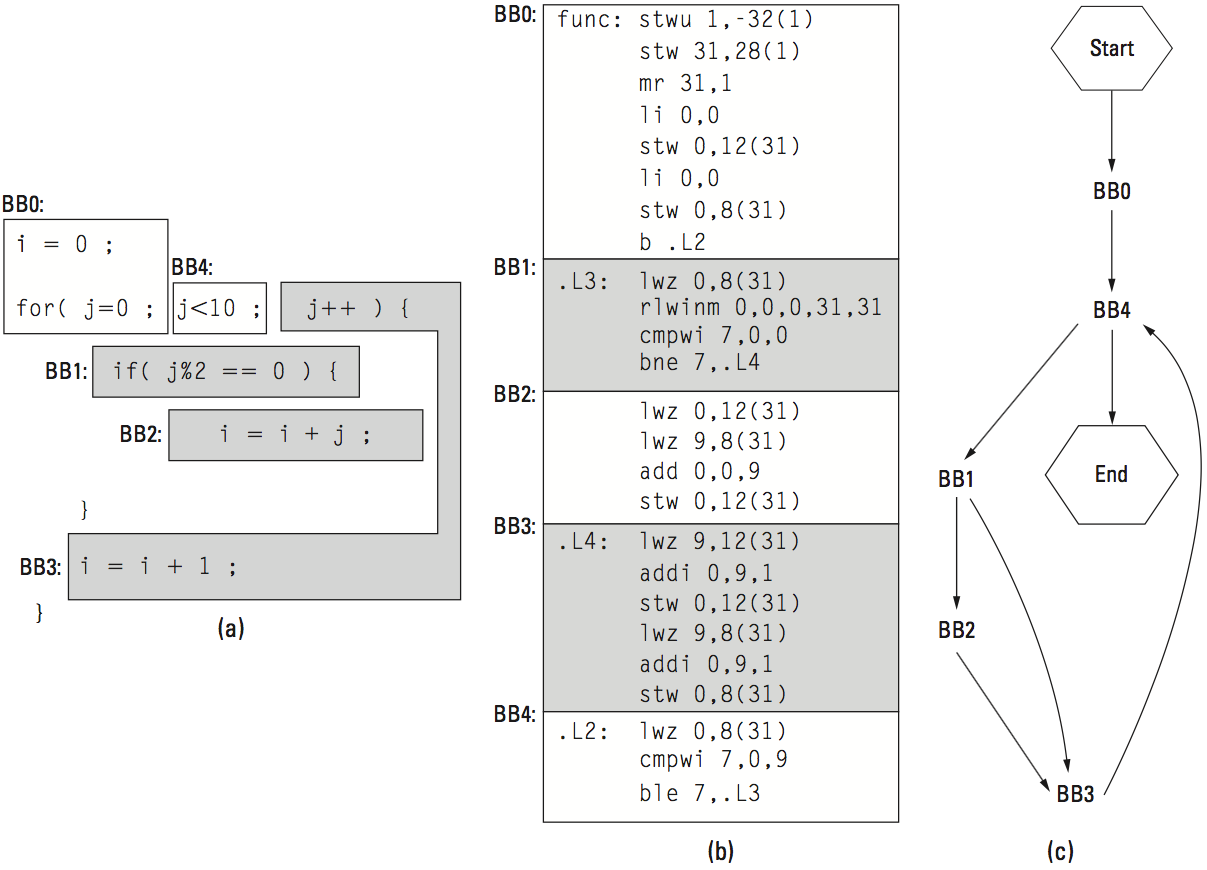
\includegraphics[width=0.35\textwidth]{img/f3-6.png}
         \caption{Identificação de blocos básicos e a representação por meio de um grafo não atrelado à uma especificação \hs.}
         \label{fig:f3-6}
      \end{figure}
      \end{comment}

      \todo{colocar isso num lugar melhro?}
      A decomposição de um DRS pode gerar dois componentes: uma porção a ser realizada em \hardware\ e; outra executada em \software.
      Essa decisão de divisão é chamada de Problema de Particionamento.
      Segundo \cite{Sass2010}, para sistemas em FPGA, o particionamento é um sub-problema de um problema mais geral no âmbito de \codesign, onde refere-se ao \design\ cooperativo entre engenheiros de \hs\ para um desenvolvimento mais eficiente.% envolvendo \textit{stakeholders}, por exemplo.
      %Para continuar, deve-se definir alguns conceitos básicos, descritos na Seção \ref{sec:gc}.

      %\subsubsection{Grafo de Chamada}
      \label{sec:gc}
         %Modelado uma sub-rotina de um DRS utilizando o GCF, definido na Seção \ref{sec:GCF}, agora será descrito uma nova notação, chamada de Grafo de Chamada (GC) utilizado para o entendimento da partição.
         Um Grafo de Chamada (GF) consiste num conjunto de GCFs, um por sub-rotinas, ou seja, $\mathcal{C} = {C_0, C_1, \dots C_{n-1}}$
         %
         %\begin{equation}
         %   \mathcal{C} = {C_0, C_1, \dots C_{n-1}}
         %\end{equation}
         %
         %onde $ C_i = (V_i, E_i) $
         onde $ C_i = (B_i, F_i) $ representa o GCF de uma sub-rotina $ i $. %, como mostrado na Equação~\ref{eq:subrotina}.
         Sendo assim, o grafo estático de chamada da aplicação é escrito por $\mathcal{A} = (\mathcal{C}, \mathcal{L}) \label{eq:a}$
         %
         %\begin{equation}
         %   \mathcal{A} = (\mathcal{C}, \mathcal{L}) \label{eq:a}
         %\end{equation}
         %
         onde \A\ representa uma aplicação específica e $ \mathcal{L} \subseteq \mathcal{C} \times \mathcal{C} $ é um subconjunto do plano cartesiano dos GCF.
         Duas sub-rotinas são relacionadas se podem ser determinadas que, no tempo de compilação, a sub-rotina $ i $ tem potencial de invocar a sub-rotina $ j $, ou seja, $ (C_i, C_j) \in \mathcal{L} $.

         %É assumido que os blocos básicos de cada sub-rotina são disjuntos, ou seja, cada bloco básico em uma aplicação pertence a exatamente um GCF.
         %Além do mais, é assumido também que um nó raiz para o GC é implícito, ou seja, uma sub-rotina é designada a iniciar a execução.
         %Nem todos os executáveis podem ser expressados nesse modelo.
         %Por exemplo, o manuseio de sinais e interrupções não são representadas e assim, não é possível determinar todos vértices $ F_i $ em uma dada sub-rotina $ C_i $ de um GCF antes da execução.
         %Uma outra forma é com o paradigma de orientação à objeto.
         %Ele depende do tempo de execução para conectar os métodos virtuais invocados e dessa forma, por \design, esse paradigma nos previne de saber todos os vértices antes da execução.
         %Para agora, será considerado que o modelo é suficiente para ser expressado em \design\ referencial de \software.

         %Um equívoco comum é de que uma definição formal de particionamento só aplica à separação de aplicação componentes de \hs, ou seja, a partição contém exatamente dois conjuntos.
         %Todavia, para fazer o problema mais tratável, é comum agrupar primeiramente operandos em recursos, ou seja, uma partição com um grande número de subconjuntos, e então mapeia esses recursos tanto em \hardware\ quanto \software.
         %Assumindo que esses recursos atuam razoavelmente bem \textit{clustered}, então a decomposição de uma aplicação em componentes de \hs\ pode ser dirigida por comparações de ganho de performance desse recurso contra outro situado no outro conjunto.

         %Definidos os conceitos prévios, será definido agora, formalmente, o conceito de uma partição.

         Com esses conceitos definidos, uma partição $ \mathcal{S} = \{S_0, S_1, \dots\} $ de um conjunto universal $ U $ é um conjunto de subconjuntos de $ U $ sendo que
         %
         \begin{gather}
            \bigcup_{S \in \mathcal{S}} S = U \label{eq:part_form_1}\\
            \forall S, S' \in \mathcal{S} | S \cap S' = \emptyset \label{eq:part_form_2}\\
            \forall S \in \mathcal{S} | \mathcal{S} \cdot S \neq \emptyset \label{eq:part_form_3}
         \end{gather}
         %
         onde a Equação~\ref{eq:part_form_1} diz que cada elemento de $ U $ é um membro de, pelo menos, um subconjunto $ S \in \mathcal{S} $, e as Equações~\ref{eq:part_form_2} e \ref{eq:part_form_3} que os subconjuntos $ S \in \mathcal{S} $ são emparelhados disjuntos e não vazio.
         Em outras palavras, cada elemento do nosso universo $ U $ termina exatamente em um dos subconjuntos de $\mathcal{S}$ e nenhum dos subconjuntos são vazios.

         Com isso é possível aplicar o formalismo à $ \mathcal{A} $ se assumirmos que nosso universo é o conjunto de todos os blocos $B$ de todas as sub-rotinas de um dispositivo \wearable, então $U$ é as partições de sub-rotinas
         %
         \begin{equation}
            U = \bigcup_{C \in \mathcal{C}} B(C) \label{eq:bigcup}
         \end{equation}
         %
         e chamaremos de partição natural da aplicação, onde
         %
         \begin{equation} \small
            \mathcal{S}  = \left \{
            \underbrace{\left \{ b_0, b_1, \dots, b_{i-1} \right \}}_{\textnormal{sub-rotina }C_0},
            \underbrace{\left \{ b_i, b_{i+1}, \dots \right \}}_{\textnormal{sub-rotina }C_1},\dots
            \underbrace{\left \{ b_j, b_{j+1}, \dots \right \}}_{\textnormal{sub-rotina }C_{n-1}}
            \right \}
         \end{equation}


          \makeatletter
          \def\@eqnnum{{\normalsize \normalcolor (\theequation)}}
           \makeatother

         %
         O propósito é reorganizar a partição de blocos básicos e então mapear cada subconjunto de ambos os \hs.
         Dessa forma, pode-se criar e remover subconjuntos não vazios, e mover blocos básicos ao redor até termos uma nova partição e assim termos um novo resultado $ \mathcal{A}’ = (\mathcal{C}’, \mathcal{L}’) $, inferido a partir da reorganização da partição $ \mathcal{X}’ $.
         O segundo passo é mapear cada subconjunto de $ \mathcal{X} $ para ambos \hs\ como é exibido abaixo

         { \small
         \begin{equation}
            \mathcal{X}'\!=\!\left \{
            \underbrace{
               \underbrace{
                  \left \{ b_0, b_1, ..., b_{i-1} \right \}
               }_{\textnormal{sub-rotina }C_0}
               ...
               \underbrace{
                  \left \{ b_j, b_{j+1}, ... \right \}
               }_{\textnormal{sub-rotina }C_{n-i}}
               ...
            }_{\textnormal{\software}}
            %\
            \underbrace{
               \underbrace{
                  \left \{ b_i, b_{i+1}, ... \right \}
               }_{\textnormal{sub-rotina }C_{n-1}}
               ...
            }_{\textnormal{\hardware}}
            \right \} \label{eq:part_final}
         \end{equation}
         }

         A seguir será explicado como a performance pode ser utilizada para guiar o particionamento.
         %Para explicar como performance pode ser utilizada para guiar o particionamento, será descrita uma métrica simples chamada taxa de execução\footnote{Taxa de execução é a velocidade na qual um sistema computacional completa uma aplicação, e em um sistema de plataforma FPGA olhamos também para o \hardware\ para melhorar sua taxa de execução.} a seguir.


   \subsection{Análise para Ganho de Performance} \label{sec:ganho_performance}
      %É parcialmente motivada pelo fato de que: \textit{a)} o ganho de performance é relativamente fácil de ser mensurado e \textit{b)} por causa de que, de todas as métricas comumente utilizadas, \speedup\ é frequentemente a mais importante.
      Diferente do mundo \software\ onde se tem análise de ordem de complexidade, em \hardware\ não possui-se um guia geral para comparação.
      O ganho de performance para aplicações em geral pode estar na acumulação de pequenos ganhos.% que deveriam ser perdido numa aplicação direta na teoria de complexidade.

      % tempo software
      Para o \software, será usado a informação de \profile\ para coletar o tempo total de execução, bem com uma fração do tempo gasto em cada sub-rotina.
      %O produto disso é a aproximação entre o tempo necessário para executar uma porção de aplicação em \software\ e usar isso como o tempo que se espera que tomará em futuras execuções.
      %É considerado uma aproximação pois é dependente dos conjuntos de dados de entrada para muitas aplicações além da existência de erros que podem impactar a performance.
      Será utilizado $ s(i) $ para representar o tempo de execução esperado para uma invocação de uma sub-rotina $ i $.

      % tempo hardware
      Precisa-se também aproximar o tempo que uma implementação equivalente em \hardware\ que iria tomar e que, em \hardware, isso é frequentemente mais preciso.
      Pra isso, uma ferramenta \textit{profiling} auxiliar à síntese poderá dar uma aproximação de acurácia de propagação de tempo.
      %Ou, se o recurso é \textit{pipelined}, o número de estágios é mais precisamente conhecido.
      %Caso o recurso inclua controle de fluxo mas não contenha nenhum \textit{loop}, pode-se considerar o caminho mais longo como uma estimativa conservativa.
      %Recursos com um número variável de iterações através de um \textit{loop} apresentam o maior obstáculo para encontrar um tempo de \hardware\ aproximado.
      %Nesse caso, implementação e \textit{profiling} com recurso em \hardware\ pode ser a única solução.
      Independente, assume-se que uma aproximação apropriada $ h(i) $ para o existente tempo de execução em \hardware, sendo $ i $ o módulo construído.

      % tempo mudanca de estado, configuracao, latencia
      Por fim, a `interfaceação' entre \hs\ requer tempo e este custo também precisa ser contabilizado.
      Pode-se aproximar deste custo pela aproximação do montante total do estado que necessita ser transferido ou o custo de configuração e latência.
      Em ambos os caso, são representados por $ m(i) $ para recursos $ i \in \mathcal{H} $, sendo $\mathcal{H}$ o conjunto de recursos do \hardware.

      % y é speedup
      Por fim, o ganho, ao comparar uma solução \hs\ contra uma solução puramente \software, é tipicamente mensurado como \speedup, Equação~\ref{eq:speedup1}.
      Utiliza-se $ \gamma $ para sua representação, permitindo comparar recursos diferentes contra outros para determinar melhores particionamentos.
      Qualquer subconjunto de blocos que não produzem um maior ganho de performance, podem ser desconsiderados, ou seja, somente $ \gamma > 1.0 $ são considerados recursos candidatos.
      %Então quando considerado se um conjunto particular de blocos básicos deveriam ser mapeados ao \hardware\ ou \software, estamos interessados em seu ganho em \speedup, ou seja
      %
      \begin{equation}
         \gamma =
         \frac{
            \textnormal{\textit{hardware speed}}
         }{
            \textnormal{\textit{software speed}}
         }
         =
         \frac{
            \frac{
               1
            } {
               \textnormal{\textit{hardware time}}
            }
         } {
            \frac{
               1
            }{
               \textnormal{\textit{software time}}
            }
         }
         =
         \frac{
            \textnormal{\textit{software time}}
         } {
            \textnormal{\textit{hardware time}}
         } \label{eq:speedup1}
      \end{equation}
      %
      Mais especificamente, interessa-se no ganho de performance individual de cada recurso e assim, definindo $ \gamma(i), i \in \mathcal{C} $
      %
      \begin{equation}
         \gamma(i) = \frac{s(i)}{h(i) + m(i)}
      \end{equation}
      %
      %onde $ h(i) $ e $ s(i) $ são o tempo de execução de uma implementação de um recurso $ i $ em \hs\ e a função $ m(i) $ é o tempo que se leva para sincronização, ou seja, o tempo que leva para guiar um dado entre o processador e o item reconfigurável.

      %Assumindo por um momento que usaremos esse recurso separado em nosso \design, deve-se questionar sobre o quão rápido é a aplicação.
      A velocidade da aplicação é dependente dos ganhos de performance do recurso e o quão frequentemente ele é utilizado no DRS.
      Pode-se ter essa fração do tempo gerado de um recurso particular $ p(i) $ a partir de informações de \textit{profile} e dessa forma o \speedup\ da aplicação no geral será
      %
      \begin{equation}
         \Gamma = \left [
         (1 - p(i))
         +
         \frac{
            p(i)
         }{
            \gamma(i)
         } \right ]^{-1}
      \end{equation}
      %
      A inversão representa que estamos movendo entre taxa de execução e tempo de execução para manter o sentido de ganho de performance.

      %A partir dessa equação, podemos observar que aumentando a velocidade do \hardware\ de um único recurso tem-se menos e menos impacto na performance da aplicação a medida que sua frequência decresce.

      %Para aumentar a performance sistêmica de uma aplicação no geral, também deve-se aumentar o sistema com múltiplos recursos que aumentará a performance de componentes individualmente assim como aumentando a fração agregada de tempo gasto em \hardware.
      Para computar o \speedup\ de múltiplos recursos em \hardware, deve-se avaliar o ganho sistêmico de um conjunto de recursos $ \mathbb{D} $.
      %Para estimar a performance desta partição, podemos adicionar recursos e rearranjar os termos para ter um ganho de performance almejado no geral,
      Assim, para o cálculo de performance dos recursos, utiliza-se da Equação \ref{eq:d_final}.
      %
      \begin{equation}
         \Gamma (\mathbb{D}) =
         \left [
         \sum _{i \in \mathbb{D}} \left (
         \frac{
            p(i)
         }{
            \gamma(i)
         }-p(i)
         \right) + 1
         \right ]^{-1} \label{eq:d_final}
      \end{equation}

      \subsubsection{A Considerações de Recursos Finitos em Componentes Eletrônicos} \label{sec:recursos}

         Uma hipótese de consideração de recursos seria adicionar esses na abordagem $\sum_i p_i$, ou seja, implementar tudo em \hardware\ para maximizar a performance, o que no caso, ignoraria todos os custos de desenvolvimento e recursos finitos.
         Entretanto, num FPGA, há um número finito de recursos disponíveis para sintetização de circuitos em \hardware\ e como tais recursos são limitados, a maioria das aplicações realísticas iriam exceder esse limite disponível. \todo{aqui entra o fpga de pequeno porte}

         Uma outra forma é contar o número de células lógicas requeridas para cada recurso.
         Um FPGA que terá um valor total escalar $ r_{FPGA} $, representará o total de números de células lógicas disponíveis para sintetização.
         Então $ r(i) $ pode ser usado para representar a quantidade de células lógicas requeridas por cada recurso $ i $.
         Fazendo uma simples relação, tem-se que $ \sum_{i \in \mathbb{D}} r(i) < r_{FPGA} $ restringe quão largo $ \mathbb{D} $ pode crescer, onde $ \mathbb{D} $ é o conjunto de recurso incluídos no \design.

         Sabendo que dispositivos modernos são heterogêneos, uma típica plataforma FPGA tem múltiplos tipos de recursos além de células lógicas como memória, blocos DSP, etc., podendo ser representados por um vetor de recursos
         %
         \begin{equation} \small
            \vec{r}_{FPGA} =
            \begin{pmatrix}
            r_{Logic\ Cells} \\
            r_{Memory}\\
            r_{DSP}\\
            \vdots \\
            r_{n-1}
            \end{pmatrix}
         \end{equation}
         %
         e com isso,
         %
         %\begin{equation}
            $\sum_{i \in \mathbb{D}} \vec{r}(i) < \vec{r}_{FPGA}$.
         %\end{equation}
         %

         %Infelizmente\todo{a}, esse modelo não leva em consideração o fato de que alguns recursos alocados podem interferir em outros, além de que a estimativa de performance é frequentemente baseada na suposição que recursos são próximos um do outro e recursos de rotas não são parte integral do modelo.
